\documentclass{beamer}
\usetheme{tokitex}

\usepackage{graphics}
\usepackage{multirow}
\usepackage{tabto}

\usepackage[english,bahasa]{babel}
\newtranslation[to=bahasa]{Section}{Bagian}
\newtranslation[to=bahasa]{Subsection}{Subbagian}

\usepackage{listings, lstautogobble}
\usepackage{color}

\definecolor{dkgreen}{rgb}{0,0.6,0}
\definecolor{gray}{rgb}{0.5,0.5,0.5}
\definecolor{mauve}{rgb}{0.58,0,0.82}

\lstset{frame=tb,
  language=pascal,
  aboveskip=1mm,
  belowskip=1mm,
  showstringspaces=false,
  columns=fullflexible,
  keepspaces=true,
  basicstyle={\small\ttfamily},
  numbers=none,
  numberstyle=\tiny\color{gray},
  keywordstyle=\color{blue},
  commentstyle=\color{dkgreen},
  stringstyle=\color{mauve},
  breaklines=true,
  breakatwhitespace=true,
  autogobble=true
}

\title{Struktur Data Dasar}
\author{Tim Olimpiade Komputer Indonesia}
\date{}

\begin{document}

\begin{frame}
\titlepage
\end{frame}

\begin{frame}
\frametitle{Pendahuluan}
Melalui dokumen ini, kalian akan:
\begin{itemize}
	\item Mengenal beberapa macam struktur data dasar
	\item Mengetahui pentingnya penggunaan struktur data
	\item Mengetahui operasi-operasi yang dapat dilakukan pada struktur data dasar
\end{itemize}
\end{frame}

\begin{frame}
\frametitle{Kilas Balik: Array}
Apakah Anda masih ingat mengenai struktur data array?
Array merupakan salah satu contoh struktur data yang dasar yang mendukung operasi berikut :
\begin{itemize}
	\item Membaca elemen didalam array secara random. Pada array, kita dapat membaca elemen pada indeks yang kita inginkan.
	\item Mengupdate elemen didalam array secara random. Pada array, kita dapat mengubah nilai elemen didalam array
\end{itemize} 
\end{frame}

\section{Linked List}
\frame{\sectionpage}

\begin{frame}
\frametitle{Mengenal Linked List}
\begin{figure}
	\centering
	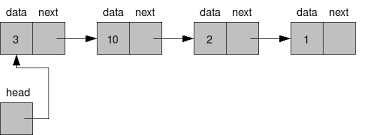
\includegraphics[width=6 cm]{asset/linkedlist.png}
\end{figure}
\begin{itemize}
	\item Linked list terdiri dari kumpulan \alert{node} yang saling terhubung
	\item Tiap node terdiri dari elemen yang akan disimpan dan \alert{pointer} ke node lainnya
	\item Pointer tersebut yang menghubungkan antar node dalam linked list
\end{itemize}
\end{frame}

\begin{frame}
\frametitle{Mengenal Linked List (lanj.)}
Berdasarkan hubungannya dengan node lain, linked list terbagi menjadi 2 macam, yaitu:
\begin{itemize}
	\item Single Linked List, yaitu linked list dimana tiap nodenya hanya memiliki pointer ke node selanjutnya saja. Tiap node hanya memiliki pointer \alert{next} untuk menunjuk node selanjutnya.
	\item Double Linked List, yaitu linked list dimana tiap nodenya memiliki pointer terhadap node selanjutnya dan node sebelumnya. Tiap pointer memiliki pointer next dan \alert{prev} untuk menunjuk node sebelumnya.
\end{itemize}
\end{frame}

\begin{frame}
\frametitle{Mengenal Linked List (lanj.)}
Selain itu, berdasarkan bentuknya, linked list juga dapat terbagi menjadi 2 macam, yaitu:
\begin{itemize}
	\item Linear Linked List, yaitu linked list dimana \alert{tail} atau node paling terakhir nextnya dihubungkan ke \alert{NULL}. Demikian pula dalam double linked list, maka \alert{head} atau node pertama prevnya dihubungkan ke NULL.
	\item Circular Linked List, yaitu linked list dimana tail bagian nextnya akan dihubungkan ke head. Selain itu, bagian prev pada head juga akan dihubungkan ke tail. 
\end{itemize}
\end{frame}

\begin{frame}
\frametitle{Keuntungan Linked List}
Mengapa kita harus menggunakan linked list? Hal ini dikarenakan linked list memiliki keuntungan dalam menangani penghapusan suatu elemen. Sebagai contoh, misal kita akan menghapus salah satu elemen pada linked list. Maka yang perlu dilakukan hanya menghapus node tersebut. Jika dibandingkan dengan array, maka penghapusan suatu elemen harus menggeser seluruh elemen setelah atau sebelum elemen yang dihapus.
\end{frame}

\begin{frame}
\frametitle{Kerugian Linked List}
Namun, penggunaan linked list juga memiliki kerugian. Sebagai contoh, untuk proses membaca elemen tidak semudah dalam pembacaan elemen pada array. Untuk membaca elemen pada indeks tertentu, maka harus dilakukan iterasi mulai dari node head hingga ke node yang diinginkan. Begitu pula dengan proses pengupdatean harus dilakukan iterasi dari awal terlebih dahulu.
\end{frame}

\section{Stack}
\frame{\sectionpage}

\begin{frame}
\frametitle{Soal Pemanasan}

Misal kita mendapat soal sebagai berikut
\begin{itemize}
	\item Anda diberikan sebuah string misal "acaabcbcd"
	\item Cari string "abc" dalam string tersebut. Jika ditemukan maka hapus string "abc" tersebut, lalu ulangi pencarian.
	\item Pencarian berakhir ketika tidak terdapat string "abc" lagi. Outputkan total penghapusan yang berhasil dilakukan
	\item Contoh, pada string "acaabcbcd" terdapat sebuah string abc, dan hapus string tersebut menjadi "acabcd". Lalu, ditemukan lagi string abc dan hapus menjadi "acd". Karena tidak ditemukan lagi string "abc", maka output 2.
\end{itemize}
\end{frame}

\begin{frame}
\frametitle{Mengenal Stack}

Stack dapat dimisalkan seperti tumpukan piring. Jika terdapat piring baru yang ingin dimasukkan, maka piring tersebut masuk dari paling atas. Jika sebuah piring akan diambil dari tumpukan, maka yang diambil juga piring yang paling atas.

\begin{figure}
	\centering
	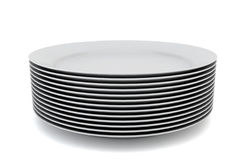
\includegraphics[width=4 cm]{asset/plates-stack.jpg}
\end{figure}

\end{frame}

\begin{frame}
\frametitle{Mengenal Stack (lanj.)}

Seperti pada analogi tumpukan piring, struktur data stack memiliki sifat yang sama:
\begin{itemize}
	\item Push, yaitu memasukan elemen baru ke bagian akhir dari stack
	\item Pop, yaitu membuang elemen paling akhir dari stack
\end{itemize}

\begin{figure}
	\centering
	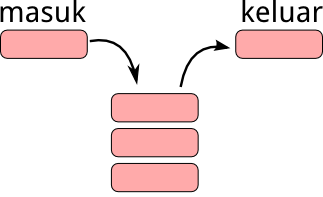
\includegraphics[width=4 cm]{asset/stack.png}
\end{figure}
\end{frame}

\begin{frame}
\frametitle{Pembahasan Soal}

Setelah mengenali struktur data stack, maka kita sudah dapat menjawab soal sebelumnya dengan efisien.
\begin{itemize}
	\item Lakukan iterasi tiap karakter pada string tersebut
	\item Untuk karakter selain huruf 'c', maka masukkan ke stack yang dimiliki
	\item jika karakter sekarang adalah 'c', maka ada kemungkinan bahwa string terakhir adalah "abc". Oleh karena itu, cek 2 elemen teratas dari stack, apakah 'b' dan 'a'.
	\item Jika tidak, maka masukkan 'c' kedalam stack.
	\item Jika iya, maka terdapat 1 penghapusan, lalu pop huruf 'b' dan 'a' dari stack.
\end{itemize}
Kompleksitas total adalah O(n) yang cukup efisien karena pada tiap karakter, kita hanya memasukkan kedalam stack atau mengecek 2 elemen teratas dari stack.
\end{frame}

\end{document}


